\documentclass[graphics]{beamer}
\usepackage{xcolor}
\usepackage{graphicx}
\usepackage{verbatim}
\usepackage{wrapfig}
\usepackage{tabularx}
\usepackage{multirow}
\usepackage{amssymb}
\usepackage{pifont}
\usepackage{tikz}
\def\Checkmark{\tikz\fill[scale=0.2](0,.35) -- (.25,0) -- (1,.7) -- (.25,.15) -- cycle;} 

\useoutertheme{shadow}
%\usecolortheme{orchid}
\usecolortheme{seahorse}
\newcommand{\cmark}{\text{\ding{51}}}
%\newcommand*{\GtrSim}{\smallrel\gtrsim}

% math commands
\newcommand{\be}{\begin{eqnarray}}
\newcommand{\ee}{\end{eqnarray}}
\newcommand{\beq}{\begin{equation}}
\newcommand{\eeq}{\end{equation}}
\def\simless{\mathbin{\lower 3pt\hbox
      {$\rlap{\raise 5pt\hbox{$\char'074$}}\mathchar"7218$}}}
\def\simgreat{\mathbin{\lower 3pt\hbox
      {$\rlap{\raise 5pt\hbox{$\char'076$}}\mathchar"7218$}}} %> or of order

% variables

\def\toonscale{0.45}
\def\mboxy#1{\mbox{\small #1}}

\defbeamertemplate*{title page}{customized}[1][]
{
  \usebeamerfont{title}\inserttitle\par
  \usebeamerfont{subtitle}\usebeamercolor[fg]{subtitle}\insertsubtitle\par
  \bigskip
  \usebeamerfont{author}\insertauthor\par
  \usebeamerfont{institute}\insertinstitute\par
  \usebeamerfont{date}\insertdate\par
  \usebeamercolor[fg]{titlegraphic}\inserttitlegraphic
}
\begin{comment}
\AtBeginSection[]{
  \frame{
    \frametitle{Outline}
    \tableofcontents[currentsection]
  }
}
\end{comment}


\title{\textcolor{white}{Fast Radio Burst Scintillation/scattering}}
%\subtitle{}
\author[U. Pen]{{
\textcolor{green}{\small Ue-Li Pen, CITA, scintillometry collaboration}
}
\\[8mm] 
}
\date{\textcolor{green}{February 14, 2017}}


\begin{document}

\frame{
\vspace{-0.5in}
\begin{center}  
%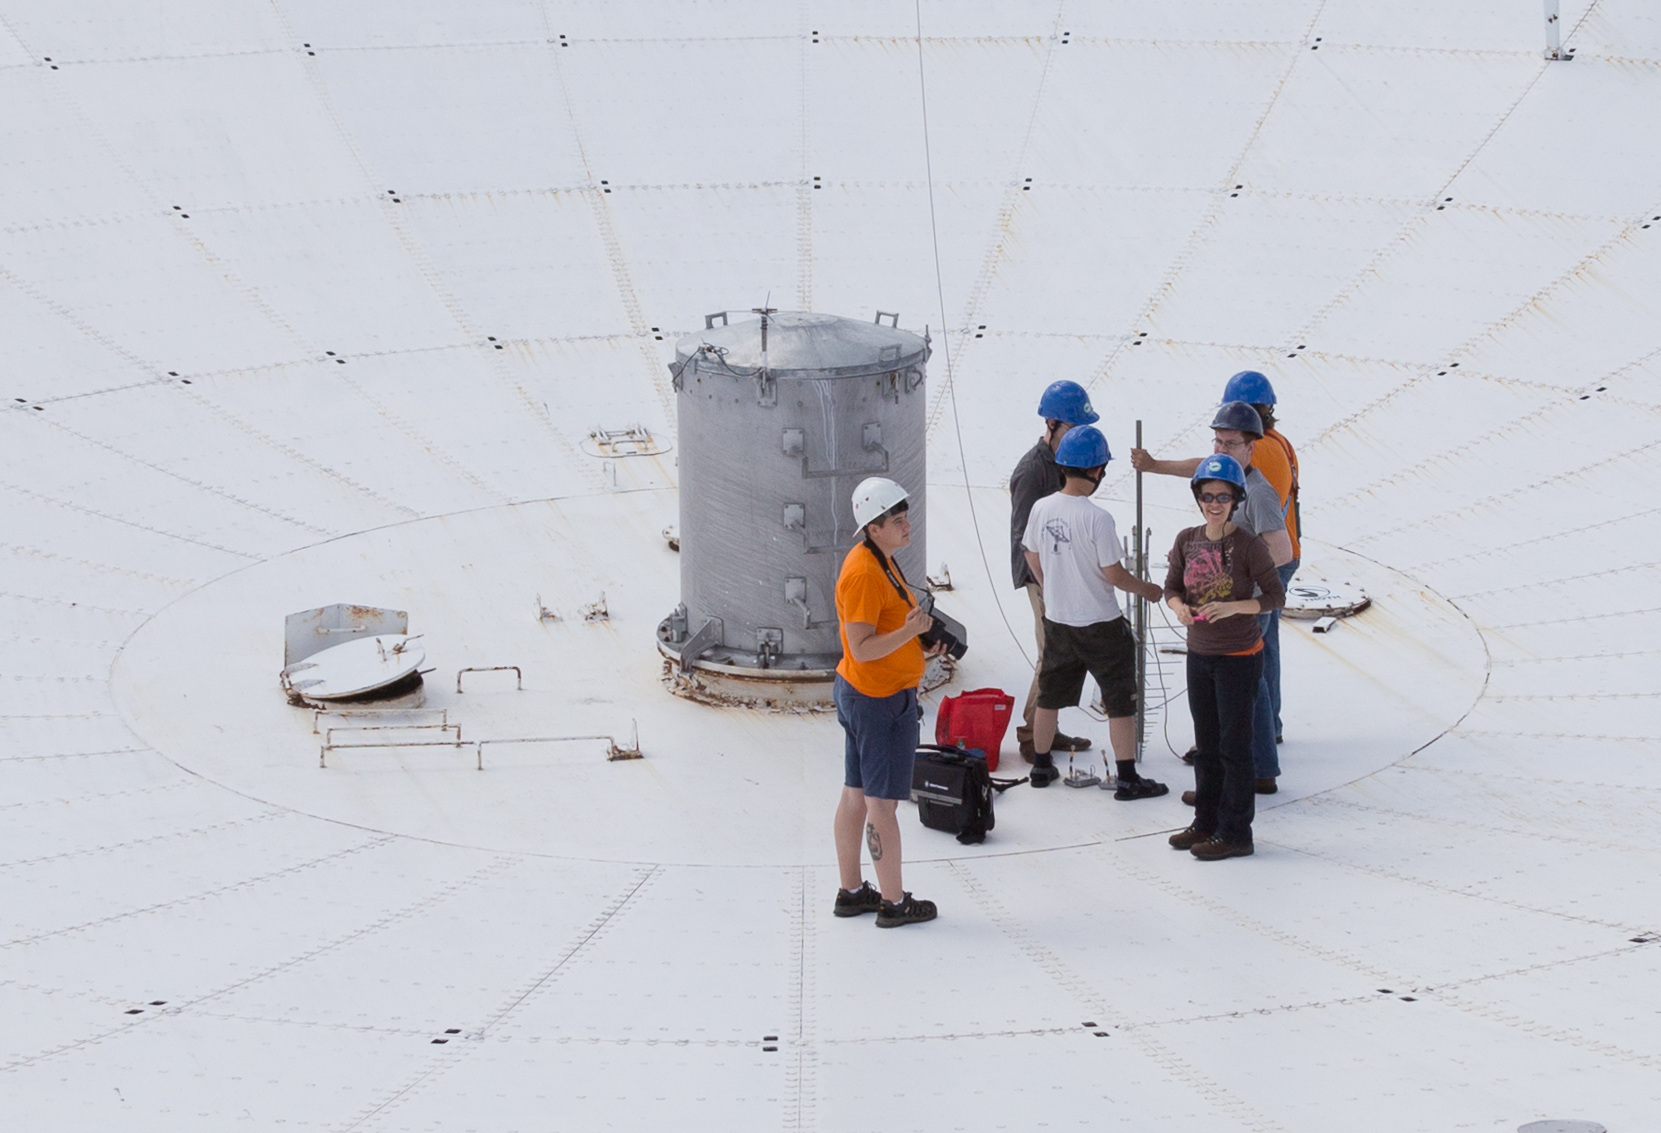
\includegraphics[width=4.4in]{Figures/IMG-0438-by-Andre-cropped.jpg}
\end{center}
\begin{picture}(320,250)
\put(-35,6){
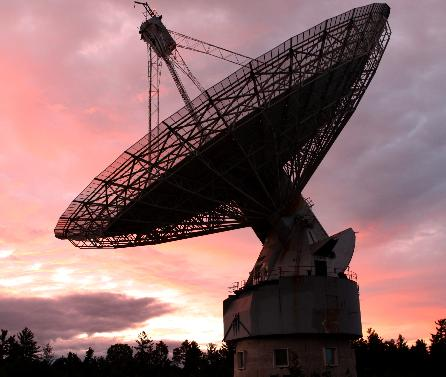
\includegraphics[width=5.1in]{Figures/IMG-7749-ARO-crop.JPG}
}
\end{picture}
\vspace{-4in}
\\
%image credit: NRAO/AUI/NSF
\\
\vspace{1in}
\titlepage
}

%\section*{Introduction}
\section{Introduction}

\begin{comment}
  \subsection{Outline}

  \frame{
    \frametitle{Outline}
    \tableofcontents
  }
\end{comment}

  \frame{
    \frametitle{Overview}
    \begin{itemize}
      \item two screen lensing
      \item FRB: scattering and scintillation
      \item FRB110523: not IGM
    \end{itemize}
  }


\frame{
    \frametitle{Crab}
     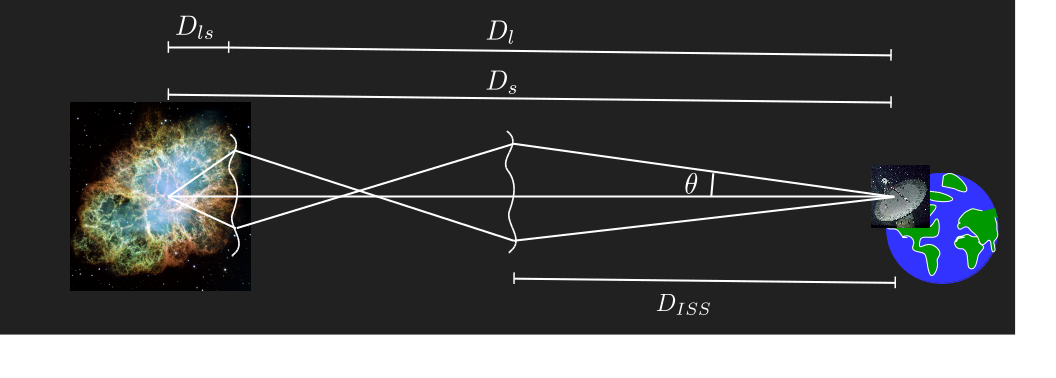
\includegraphics[width=1.1\textwidth]{Figures/TwoScreenGeometry.png}

(figure credit: R. Main)
}

\section{FRBs}


\frame{
    \frametitle{FRB110523}
     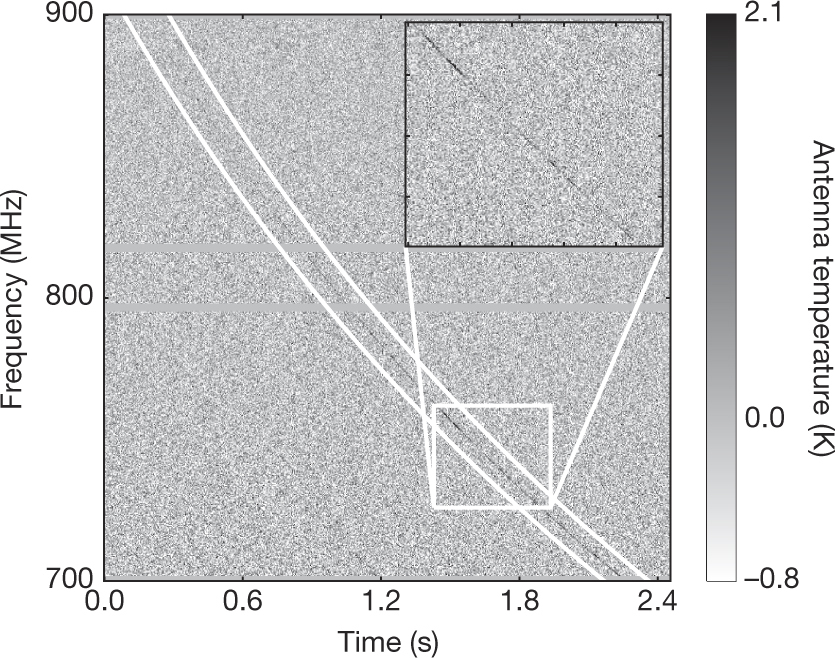
\includegraphics[width=0.8\textwidth]{Figures/nature15769-f1.jpg}

Masui et al 2015
}

  \frame{
    \frametitle{FRB110523}
    \begin{itemize}
    \item Masui et al 2015
    \item  recorded on May 23, 2011
     \item part of GBT-IM survey, for 21cm intensity mapping (Chang et al 2010,
       Nature, 466, 463)
     \item first example of 21cm/FRB synergy, c.f. CHIME-FRB, APERTIF, etc
    \end{itemize}
  }

  \frame{
    \frametitle{Two screen physics}
    \begin{itemize}
      \item FRB110523:
      \item long $\sim 1$ms: local to host
      \item short $\sim 1 \mu$s: galactic
      \item FRB121102:
      \item long $\sim 10$ns: local to host
      \item short $\sim 20 \mu$s: galactic
    \end{itemize}
  }
\frame{
    \frametitle{Scattering}
     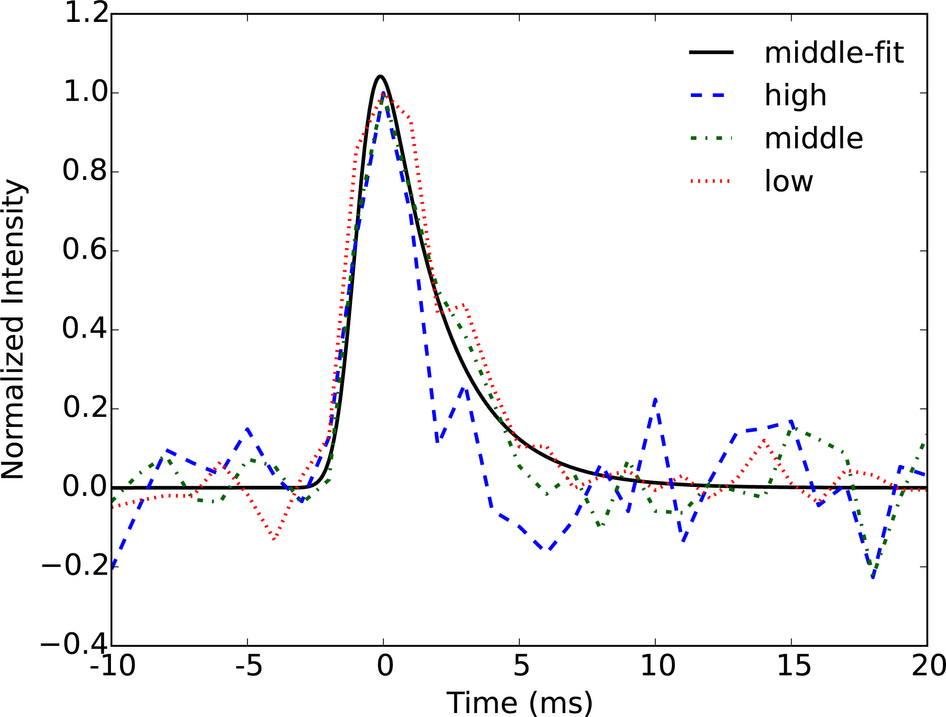
\includegraphics[width=0.8\textwidth]{Figures/nature15769-sf2.jpg}
}
  \frame{
    \frametitle{interpretation}
    \begin{itemize}
    \item ms scattering is generally due multipath propagation
    \item location was once thought to be IGM or intervening halos
    \item FRB110523 shows $\mu$s scintillation from Galactic multipath
    \item scattering tail scintillates!
    \item {\it stars twinkle, planets don't}
    \item constrains source size less than $\sim$ microarcsecond
    \item scattering screen is physically associated with FRB, not
      intergalactic or intervening
    \end{itemize}
  }

\section{Summary}



  \frame{
    \frametitle{Conclusion}
    \begin{itemize}
      \item Two screen scintillation/scattering: crab, FRB110523
      \item possible cause of spectral structure in FRB121102
      \item low frequency VLBI quantifies galactic screen distance,
        constrain source screen distance
      \item DISS could be due to refractive interference, not turbulence
        (Goldreich\&Sridhar 2006, UP\&Levin 2014)
      \item galactic centre magnetar (and maybe crab) important example for
        understanding FRBs
      \item ISM structure: mapping cosmic plasma and magnetic fields
      \item always trigger and store baseband data!
    \end{itemize}
  }

\end{document}
